\documentclass[11pt]{exam}
\usepackage{graphicx} % Required for inserting images
\usepackage{amssymb}
\usepackage{amsmath}
\usepackage{optidef}
\usepackage{listings}
\usepackage{xcolor} % for custom colors
\usepackage{minted} % for code
\usepackage[T1]{fontenc}

% === Make things tighter ===
\usepackage[margin=0.75in]{geometry} % <- widen/narrow by changing 1.25in
\usepackage{setspace}
% \setstretch{0.95} % line spacing
\usepackage{enumitem}
% \setlist{nosep}  % removes vertical space around lists
% \setlist[itemize]{topsep=3pt, itemsep=3pt, parsep=1pt, partopsep=0pt}
% \setlist[enumerate]{topsep=3pt, itemsep=3pt, parsep=1pt, partopsep=0pt}
\usepackage{titlesec}
% \titlespacing*{\section}{0pt}{4.0ex plus 0.5ex minus 0.5ex}{0.8ex}
% \titlespacing*{\subsection}{0pt}{3.0ex plus 0.3ex minus 0.3ex}{0.6ex}
% \titlespacing*{\subsubsection}{0pt}{2.0ex plus 0.2ex minus 0.2ex}{0.4ex}
% \titlespacing*{\paragraph}{0pt}{1.5ex plus 0.2ex minus 0.2ex}{0.4ex}
\newcommand{\todo}[1]{\textit{\textcolor{orange}{ [#1]}}}
\qformat{\textbf{Problem \thequestion\ (\thequestiontitle)}\hfill}


\lstset{
  language=Python,
  basicstyle=\ttfamily\scriptsize,
  keywordstyle=\color{blue},
  stringstyle=\color{red},
  commentstyle=\color{gray},
  showstringspaces=false,
  frame=single,
  breaklines=true
}
\title{6.S974 Games, Learning, and Security\\\large HW2}
\author{Erich Trieschman}
\date{\today}
\begin{document}
\maketitle

\begin{questions}
    \titledquestion{Cybersecurity with Incomplete Information}
    \begin{parts}
        \part \textbf{Pure strategies.} A strategy specifies a choice for each type. 
        \begin{itemize}
            \item Attacker $(\theta_1=4, \theta_1=8)$: $\{(A,A), (A,N), (N,A), (N,N)\}$
            \item Company: $(\theta_2=1, \theta_2=3)$: $\{(P,P), (P,U), (U,P), (U,U)\}$
        \end{itemize}
        A strategy profile is a tuple of one pure strategy per player. In this case each player has four pure strategies, so there are $4\times4 = 16$ strategy profiles.
        
        
        \part \textbf{Prior and beliefs.} Types are equally likely to occur and independent so
        \begin{align*}
         p(\theta_1,\theta_2) = \tfrac12 \times \tfrac12 = \tfrac14,
         \qquad\forall\;\theta_1,\;\forall\;\theta_2
        \end{align*}
        Beliefs are conditional on the attacker or the company's types
        \begin{align*}
            \mu_1(\theta_2=1 \mid \theta_1 = 4) = \frac{p(4,1)}{p(4,1) + p(4,3)} = \frac{\tfrac14}{\tfrac14 + \tfrac14} = \tfrac12
        \end{align*}
        Because the prior is uniform over $(\theta_1,\theta_2)$, this belief holds for every player's type for every other player's type so
        \begin{align*}
            \mu_1(\theta_2 \mid \theta_1) = \mu_2(\theta_1 \mid \theta_2) = \tfrac12
        \end{align*}

        \part \textbf{Pure strategy best response.}
        Expected payoff when company plays $P$ is $E_{A \sim\alpha}[u_2(P,A)] = -\alpha\theta_2 - (1-\alpha)\theta_2 = -\theta_2$ and when company plays $U$ is $E_{A \sim\alpha}[u_2(U,A)] = -4\alpha$, so
        \begin{align*}
            BR_2(\alpha) = \begin{cases}
                P & \theta_2 < 4\alpha\\
                \{P,U\} & \theta_2 = 4\alpha\\
                U & \text{else}
            \end{cases}
            \implies \begin{cases}
                (P,P) & \alpha \ge \tfrac34\\
                (P,U) & \tfrac14\leq \alpha \leq \tfrac34 \\
                (U,P) & \text{never}\\
                (U,U) & \alpha\le\tfrac14\\
            \end{cases}
        \end{align*}
        And for the attacker we get $E_{P\sim\pi}[u_1(P,A)] = -\pi + (1-\pi)(\theta_1 - 1) = (1-\pi)\theta_1 - 1 $ 
        and $E_{P\sim\pi}[u_1(P,N)] = 0$
        \begin{align*}
            BR_1(\pi) = \begin{cases}
                A& \pi < 1 - \frac{1}{\theta_1}\\
                \{A,N\} & \pi = 1 - \frac{1}{\theta_1}\\
                N & \text{else}
            \end{cases}
            \implies \begin{cases}
                (A,A) & \pi \le \tfrac34\\
                (A,N) & \text{never}\\
                (N,A) & \tfrac34 \le \pi \le \tfrac78\\
                (N,N) & \pi \ge \tfrac78\\
            \end{cases}
        \end{align*}

    \part\textbf{Does a pure strategy Bayes Nash Equilibrium exist?}
    \begin{itemize}
        \item Begin with attacker pure strategy $(A,A)$: $\sigma_1(A\mid \theta_1=4) = 1 = \sigma_1(A\mid\theta_1=8)$ so $\alpha = 1$. From part (c) $BR_2(1) = (P,P)$.
        By the same logic company pure strategy $(P,P)$ yields $\pi = 1$ $BR_1(1) = (N,N)$.
        Repeating, attacker pure strategy $(N,N)$ yields $\alpha = 0$ and $BR_2(0) = (U,U)$. 
        Company pure strategy $(U,U)$ yields $\pi=0$ and $BR_1(0)=(A,A)$, returning us to the start of the cycle. So there's no pure strategy Bayes Nash Equilibrium with any combination of $((A,A), (N,N))$ and $((P,P),(U,U))$
        \item Take attacker pure strategy $(A,N)$ yielding $\alpha=\tfrac12$ and $BR_2(\tfrac12)=(P,U)$. The company's best response yields $\pi=\tfrac12$ and $BR_1(\tfrac12)=(A,A)$, returning us to the first cycle. 
        \item Take attacker strategy $(N,A)$ yielding $\alpha=\tfrac12$. This produces the same $BR_2(\tfrac12)=(P,U)$ above returning us to the first cycle.
    \end{itemize}
    Hence by process of elimination, there is no pure strategy Bayes Nash Equilibrium.

    \part\textbf{Bayesian Nash Equilibrium in behavioral strategies.}

    \paragraph{Necessary condition $\pi=\tfrac34$}
    By contradiction suppose $\pi\neq\tfrac34$ in equilibrium. Recall that a mixed action is a best response only if every action in its support is a pure best response by theorem. 
    
    \paragraph{Case 1 ($\pi>3/4$).}
    For any $\pi > 3/4$ attacker type $\theta_1=4$ has only a pure best response $N$ (because mixed best response requires pure best response in its support) and $\sigma_1(A\mid\theta_1=4) = 0$. So $\alpha = \sigma_1(A\mid\theta_1=8)/2$, which implies $\alpha \leq 1/2$.

    For any $\alpha \leq 1/2$ the company type $\theta_2=3$ has only a pure best response $U$ and $\sigma_2(P\mid\theta_2=3)=0$. So $\pi = \sigma_2(P\mid\theta_2=1)/2$, which implies $\pi \leq 1/2$, a contradiction to $\pi > 3/4$.    
    
    \paragraph{Case 2 ($\pi < 3/4)$}
    For any $\pi < 3/4$ the attacker has only a pure best response $(A,A)$ and $\alpha = 1$. For $\alpha = 1$ the company has only a pure best response $(P,P)$ and $\pi = 1$, contradicting $\pi < 3/4$. 

    Therefore if there exists a Bayesian Nash Equilibrium a necessary condition would be $\pi = 3/4$.

    \paragraph{Mixed strategy.}
    The probability of protecting $\pi = 3/4$ gives $\sigma_2(P\mid 1) + \sigma_2(P\mid 3) = 3/2$,
    which implies at least one company type randomizes, since pure company strategies give $\sigma_2(P\mid 1) + \sigma_2(P\mid 3) \in \{0, 1, 2\}$.

    Moreover, for $\pi = 3/4$ the best response of attacker type $\theta_1=8$ is $A$, implying a probability of attack $\alpha \geq 1/2$. 

    For the company to have a mixed strategy and $\alpha \geq 1/2$, it must be that $\alpha = 3/4$ so that the mixed strategy best response can have a support greater than 1: the company type $\theta_1=3$ is indifferent at $\alpha=3/4$ and type $\theta_1=1$ is not.

    This support tells us that company type $\theta_2=1$ has a pure strategy best response of $P$ and $\sigma_2(P\mid 1) = 1$. Plugging this into our equation for $\pi$ above we get $\sigma_2(P\mid 3) = 1/2$.

    Note that $\sigma_1(A\mid8) = 1$ follows directly from attacker type $\theta_1=8$'s best response of $A$. Solving $\alpha = 3/4 = (1 + \sigma_1(A\mid4))/2$ gives $\sigma_1(A\mid4)= 1/2$.  

    Therefore if there is a mixed strategy Bayesian Nash Equilibrium it must be that
    \begin{align*}
        \sigma_2(P\mid 3) = 1/2 = \sigma_1(A\mid4),\quad \sigma_2(P\mid1) = 1 = \sigma_1(A\mid8).
    \end{align*}
    Suffice to validate.

    \paragraph{Validation.}
    From definition, the strategy profile is a Bayes Nash Equilibrium if for every player and every type the strategy is a best response. 
    At the candidate profile $\pi = 3/4$ and $\alpha = 3/4$.
    \begin{align*}
        \operatorname{supp}(\sigma_1(\cdot\mid\theta_1=4)) = \{A,N\} &\subseteq BR_1(\tfrac34\mid\theta_1=4) = \{A,N\}\\
        \operatorname{supp}(\sigma_1(\cdot\mid\theta_1=8)) = \{A\}   &\subseteq BR_1(\tfrac34\mid\theta_1=8) = \{A\}\\
        \operatorname{supp}(\sigma_2(\cdot\mid\theta_2=1)) = \{P\}   &\subseteq BR_2(\tfrac34\mid\theta_2=1) = \{P\}\\
        \operatorname{supp}(\sigma_2(\cdot\mid\theta_2=3)) = \{P,U\} &\subseteq BR_2(\tfrac34\mid\theta_2=3) = \{P,U\}
    \end{align*}
    Each condition above was necessary for equilibrium, so it is the unique BNE.
    \end{parts}
    

    \titledquestion{Signaling through Safety Certification}
    \begin{parts}
        \part \textbf{Game tree.}
        \begin{figure}[htbp]
            \centering
            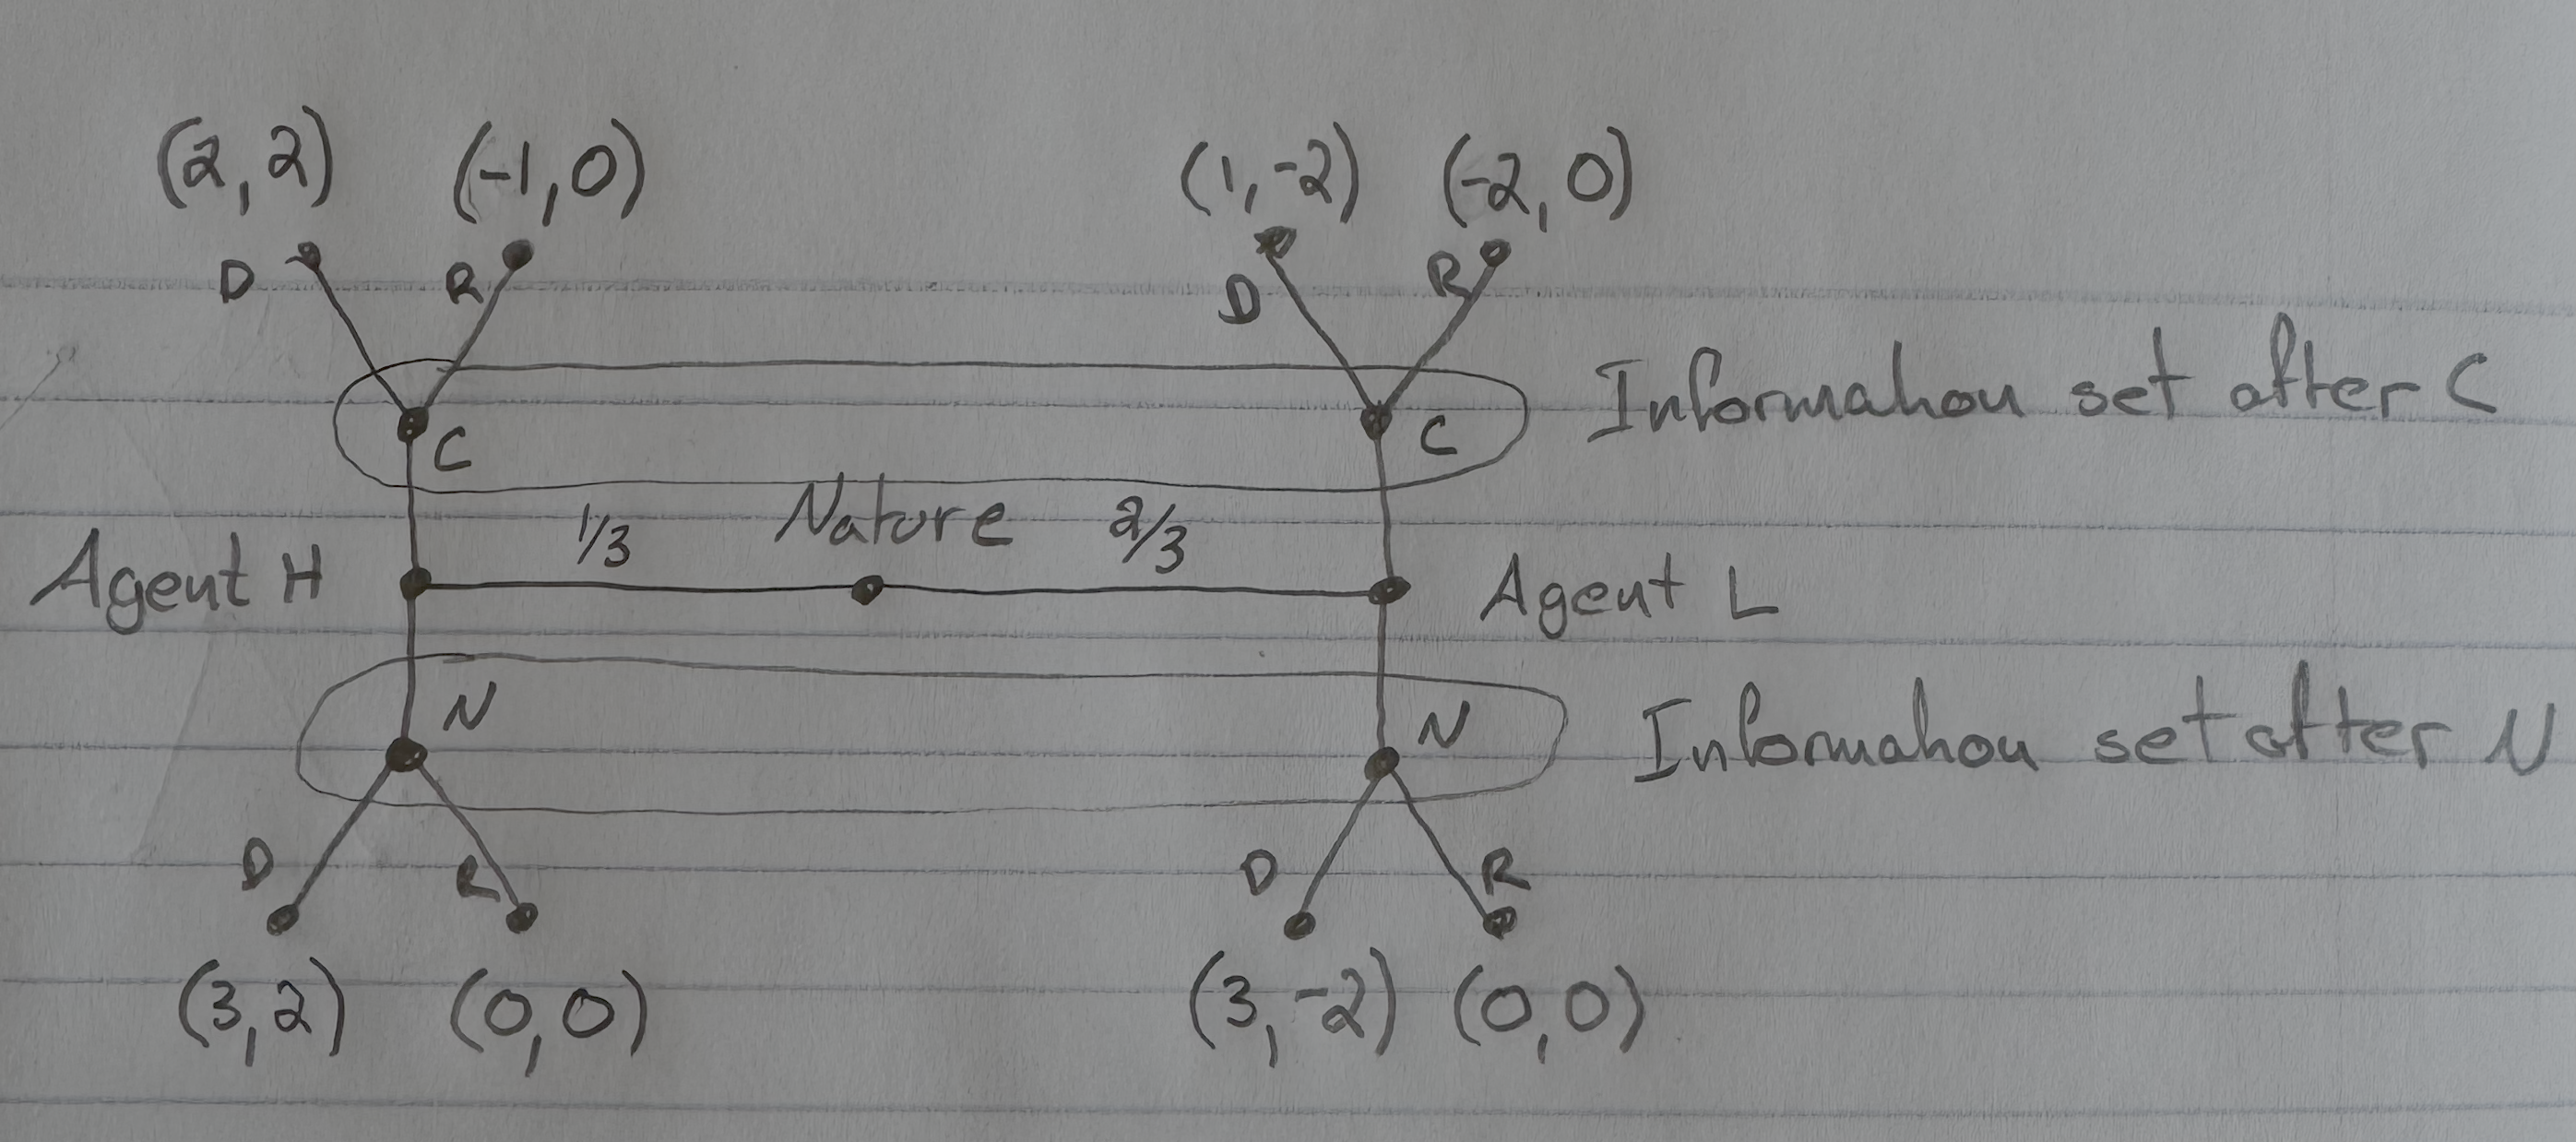
\includegraphics[width=0.6\textwidth]{hw2_problem2_parta.png}
            \caption{Problem 2 Part (a) game tree}
            \label{fig:1-a}
        \end{figure}
        \part \textbf{Does a separating PBE exist?}
        A separating PBE exists if a strategy profile $(s^*, \mu^*)$ satisfies
        \begin{enumerate}
            \item \emph{Sequential rationality.} At every information set $I$ each player's continuation strategy $s_i^*\big|_I$ maximizes expected payoff given beliefs $\mu_i^*(\cdot \mid I)$ and the other players' continuation strategies $s_{-i}^*\big|_I$.
            \item \emph{Belief consistency.} At information sets $I$ reached with positive probability, beliefs $\mu_i^*(\cdot\mid I)$ are obtained from the prior and equilibrium strategies $s^*$ using Bayes' rule.
            \item \emph{Separating.} Each provider type chooses a different signal.
        \end{enumerate}
        Candidate provider strategy profiles are $s_1(H,L) \in \{(C,N), (N,C)\}$. 
        
        \paragraph{Profile $(C,N)$.}
        Under belief consistency the operator's beliefs $\mu_2(\cdot\mid m_1)$ are
        \begin{align*}
            \mu_2(H\mid C) = \frac{P(C\mid H)P(H)}{P(C\mid H)P(H) + P(C\mid L)P(L)} 
            = \frac{1*1/3}{1*1/3 + 0} = 1, && \mu_2(L\mid C) = 0,\\
            \mu_2(H\mid N) = 0, && \mu_2(L \mid N) = 1.
        \end{align*}
        Under sequential rationality, the operator's strategy is $s_2(C) = D$ and $s_2(N) = R$.
        
        In equilibrium, the provider should not have an incentive to deviate. When $\theta_1 = H$, selecting $N$ decreases provider payoff from $2\to 0$. When $\theta_1 = L$, selecting $C$ increases provider payoff from $0\to1$. So $(C,N)$ is not a separating PBE.

        \paragraph{Profile $(N,C)$.}
        Operator beliefs are
        \begin{align*}
            \mu_2(H\mid C) = 0, && \mu_2(L\mid C) = 1, &&
            \mu_2(H\mid N) = 1, && \mu_2(L \mid N) = 0.
        \end{align*}
        The operator's strategy is $s_2(C) = R$ and $s_2(N) = D$. 
        When $\theta_1=H$, selecting $C$ decreases provider payoff from $3\to-1$. When $\theta_1=L$, selecting $N$ increases provider payoff from $-2\to3$. So $(N,C)$ is not a separating PBE.

        Therefore, there does not exist a separating PBE. 


        \part \textbf{Pooling PBE.}
        Now consider a pooling PBE where $s_1(H) = s_1(L) = N$. 
        
        The operator's beliefs are
        \begin{align*}
            \mu_2(H\mid N) = \frac{P(N\mid H)P(H)}{P(N\mid H)P(H) + P(N\mid L)P(L)} = \frac{1*1/3}{1*1/3 + 1*2/3} = 1/3, && \mu_2(L\mid N) = 2/3.
        \end{align*}
        
        The operator's strategy is based on expected payoffs
        \begin{align*}
            E_{\theta_1}[u_2(N,R\mid\theta_1)] = 0, && E_{\theta_1}[u_2(N,D\mid\theta_1)] = 1/3 * 2 + 2/3 * (-2) = -2/3
        \end{align*}
        and its strategy is $s_2(N) = R$. 

        Bayes rule cannot determine $\mu_2(\cdot\mid C)$. Let $\mu_2 := \mu_2(H\mid C)$ and ask what beliefs can discourage both provider types from deviating from $N$:
        \begin{align*}
            E_{\theta_1}[u_2(C,R\mid\theta_1)] = 0, && E_{\theta_1}[u_2(C,D\mid\theta_1)] = \mu_2 * 2 + (1-\mu_2) * (-2) = 4\mu_2 -2.
        \end{align*}
        Comparing the two expected payoffs we see for any $\mu_2 \le 1/2$ the operator's best response would be $s_2(C) = R$. Choose $\mu_2 = 0$ so $s_2(N) = s_2(C) = R$ and examine the provider's best response.

        When $\theta_1=H$, selecting $C$ decreases payoffs from $0\to-1$ and when $\theta_1=L$, selecting $C$ decreases payoff from $0\to-2$. 

        Therefore the profile $s^* = (s_1(H) = s_1(L) = N, s_2(C) = s_2(N)=R)$, together with beliefs $\mu_2(H\mid N) = 1/3$ (from Bayes' rule) and $\mu_2(H\mid C) = 0$ (chosen), is a pooling PBE.

        \part \textbf{Behavioral strategy for a semi-separating equilibrium.}

        Suppose $\sigma_1(C\mid H) = 1,\; \sigma_1(C\mid L) = p\in(0,1)$. 
        
        \paragraph{Operator beliefs.}
        \begin{align*}
            \mu_2(H\mid C) = \frac{\sigma_1(C\mid H)P(H)}{\sigma_1(C\mid H)P(H) + pP(L)}
             = \frac{1*1/3}{1*1/3 + 2p/3} = \frac{1}{1+2p}, && \mu_2(L\mid C) = \frac{2p}{1 + 2p}\\
             \mu_2(H\mid N) = 0,&& \mu_2(L\mid N) = 1.
        \end{align*}
        \paragraph{$\mathbf{\sigma_2(\cdot\mid N)}.$}
        When the provider plays $N$ the operator has a pure best response of $s_2(N) = R$ since 
        \begin{align*}
            E_{\theta_1}[u_2(N,D\mid \theta_1)] = 0*2 + 1*(-2) < 0 = E_{\theta_1}[u_2(N,R\mid \theta_1)]
        \end{align*}
        So $\sigma_2(R\mid N) = 1 = 1- \sigma_2(D\mid N)$.

        \paragraph{$\mathbf{\sigma_1(\cdot\mid L)}.$}
        When the provider plays $C$, the operator can play a mixed strategy only if both pure strategies are in its best response. This occurs when
        \begin{align*}
            E_{\theta_1\sim\mu_2}[u_2(C,D\mid \theta_1)] &= 0 
                = E_{\theta_1\sim\mu_2}[u_2(C,R\mid \theta_1)]\\
             2*\mu_2(H\mid C) + -2*\mu_2(L\mid C) &=0\\
             2/(1 + 2p) - 4p/(1 + 2p) &= 0\\
             p &= 1/2
        \end{align*}
        So $\sigma_1(C\mid L) = 1/2 = \sigma_1(N\mid L)$.

        \paragraph{$\mathbf{\sigma_2(\cdot\mid C)}$.}
        Let $\sigma_2(D\mid C) = q$ and recall $\sigma_2(R\mid N) = 1$. For a behavioral strategy equilibrium we must find $q$ such that the provider of type $\theta_1=L$ is indifferent between actions $C$ and $N$:        
        \begin{align*}
            E_{\sigma_2}[u_1(C,\sigma_2\mid L)] &= E_{\sigma_2}[u_1(N,\sigma_2\mid L)]\\
            q*1 + (1-q)(-2) &= 0 = u_1(N,R \mid L)\\
            q &= 2/3
        \end{align*}
        So $\sigma_2(D\mid C) = 2/3 = 1 - \sigma_2(R\mid C)$.

        \paragraph{$\mathbf{\sigma_1(\cdot\mid H)}$}
        It suffices to show $\sigma_1(C\mid H) = 1 = 1-\sigma_1(N\mid H)$ is a best response:
        \begin{align*}
            E_{\sigma_2}[u_1(C, \sigma_2\mid H)] &= 2/3 * 2 + 1/3(-1) = 1
            \ge 0 = E_{\sigma_2}[u_1(N, \sigma_2\mid H)]
        \end{align*}
        So $s_1(H) = C$ is a pure strategy best response confirming the check.  

        \paragraph{Equilibrium.}
        Therefore the following strategy profile
        \begin{align*}
            \sigma_1(C\mid H) = 1, \quad \sigma_1(N\mid H) = 0,\quad \sigma_1(C\mid L) = 1/2,\quad \sigma_1(N\mid L) = 1/2.\\
            \sigma_2(D\mid C) = 2/3, \quad \sigma_2(R\mid C) = 1/3,\quad \sigma_2(D\mid N) = 0,\quad \sigma_2(R\mid N) = 1.
        \end{align*}
        with beliefs
        \begin{align*}
            \mu_2(H\mid C) = 1/2, && \mu_2(L\mid C) = 1/2\\
             \mu_2(H\mid N) = 0,&& \mu_2(L\mid N) = 1.
        \end{align*}
        is a PBE in behavioral strategies.

        \paragraph{Probability of unreliable and deployed.}
        \begin{align*}
            P(D, L) &= P(D\mid L)P(L)\\
            & = \big[P(D\mid L,C)P(C\mid L) + P(D\mid L,N)P(N\mid L)\big]P(L) \tag{law of total probability}\\
            &= \big[\sigma_2(D\mid C)\sigma_1(C\mid L) + \sigma_2(D\mid N)\sigma_1(N\mid L)\big]P(L) \tag{plugging in strategy profiles}\\
            &= \big[\tfrac23\cdot \tfrac12 + 0\cdot\tfrac12\big]\tfrac23\\
            &=\tfrac{2}{9}
        \end{align*}
    \end{parts}

    \titledquestion{Traffic routing problem}
    \begin{parts}
        \part \textbf{Waldrop equilibrium.}
        \part \textbf{Mean-posterior identity.}
        \part \textbf{Public signal rule.}
        \part \todo{update}
        \part \todo{update}
        \part \todo{update}
    \end{parts}

    \titledquestion{Employment recommendations}
    \begin{parts}
        \part \todo{update}
        \part \todo{update}
        \part \todo{update}
        \part \todo{update}
    \end{parts}

    


    

    
\end{questions}
\end{document}